\documentclass{beamer}
\usetheme{default}
\usepackage{amsmath, amsfonts, amsthm} % basic math packages
\usepackage{tikz} % for making illustrations
\usetikzlibrary{shapes.arrows, arrows, decorations.markings, positioning}
\tikzset{cross/.style={path picture={
			\draw[black]
			(path picture bounding box.south east)--(path picture bounding box.north west)
			(path picture bounding box.south west)--(path picture bounding box.north east);
}}}
\usetikzlibrary{calc}
\usetikzlibrary{3d}
\usepackage{graphicx} % for importing images
\usepackage{xcolor} % more color options
\usepackage{colortbl}
\usepackage{multicol} % for making two-column lists
\usepackage{hyperref} % for hyperlinking
%\hypersetup{colorlinks=true, urlcolor=cyan,}
\usepackage{mathabx}
\usepackage{cleveref}
\usepackage{subfig}
\usepackage{array}
\usepackage{wrapfig}
\usepackage{bbm}
\usepackage{fancyhdr}
\usepackage{algorithm, algorithmicx, algpseudocode}
\usepackage{stmaryrd}
\usepackage{physics}
\AtBeginSection[]
{
	\begin{frame}
		\frametitle{Table of Contents}
		\tableofcontents[currentsection]
	\end{frame}
}

\title{A \LaTeX'ed solution to 2D Spatial Indexing.}
\author{Mitchell Scott (mtscot4)}
\begin{document}
	\begin{frame}[plain]
		\maketitle
	\end{frame}
	\begin{frame}{2D Spatial Indexing Examples}
		\tableofcontents
	\end{frame}
	\section{Assignment 4-1: Quad Trees}
	\begin{frame}{Quad-Tree Set-up}
		Insert the following points (in this order) into an initially empy Quad-Tree:
		\begin{align*}
			A = (0,0), B = (10,10), C &= (8,2), D = (9,3), E = (2,2),\\
			F = (6,2), G = (2,10), H &= (7,3), I = (5,5), J = (7,4)
		\end{align*}
		The maximum page capacity of this Quad-Tree is 4.
		\begin{itemize}
			\item Draw the current Quad-tree after each split.
		\end{itemize}
	\end{frame}
	\begin{frame}{The initially empty Quad-tree has one entry that covers the entire data space, by definition. We decided to make it $[-1,12]\times [-1,12]$.}
		\begin{center}
				
\begin{tikzpicture}
				\draw[step=0.5cm,gray,very thin] (-1,-1) grid (5.5,5.5);
				\draw[thick,-] (-1,-1) -- (5.5,-1);
				\draw[thick,-] (5.5,-1) -- (5.5,5.5);
				\draw[thick,-] (5.5,5.5) -- (-1,5.5);
				\draw[thick,-] (-1,5.5) -- (-1,-1);
			\end{tikzpicture}
		\end{center}
		
	\end{frame}
	\begin{frame}{Since the page capacity is 4, we are able to add $A,B,C,$ and $D$ with no hiccups.}
		\begin{center}
			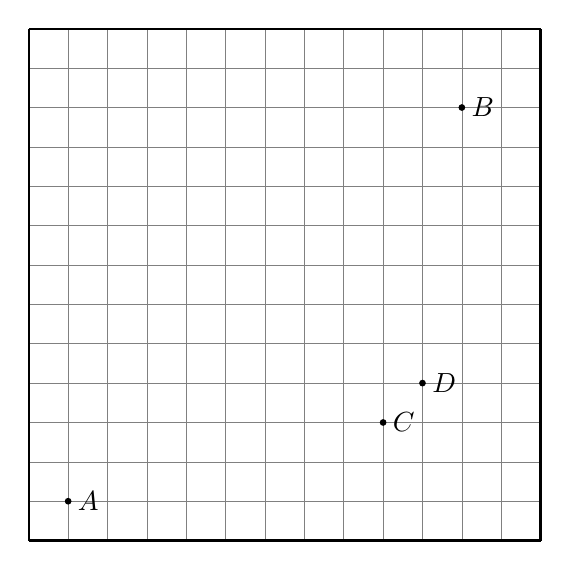
\begin{tikzpicture}
				\draw[step=0.5cm,gray,very thin] (-1,-1) grid (5.5,5.5);
				\draw[thick,-] (-1,-1) -- (5.5,-1);
				\draw[thick,-] (5.5,-1) -- (5.5,5.5);
				\draw[thick,-] (5.5,5.5) -- (-1,5.5);
				\draw[thick,-] (-1,5.5) -- (-1,-1);
				\filldraw[black] (-0.5,-0.5) circle (1pt) node[anchor=west]{$A$};
				\filldraw[black] (4.5,4.5) circle (1pt) node[anchor=west]{$B$};
				\filldraw[black] (3.5,0.5) circle (1pt) node[anchor=west]{$C$};
				\filldraw[black] (4,1) circle (1pt) node[anchor=west]{$D$};
			\end{tikzpicture}
		\end{center}
	\end{frame}
	\begin{frame}{{\bf Overflow!} Adding Point $E$, means that we will have 5 points in the data space, which is higher than 4. Therefore we have to do a quad-split.}
		\begin{center}
			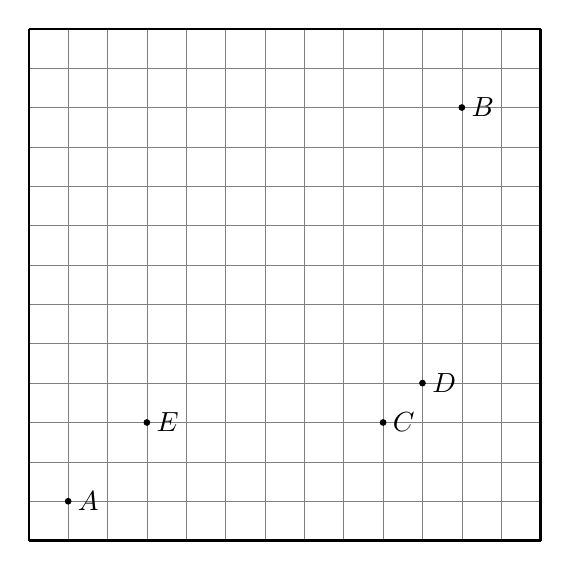
\begin{tikzpicture}
				\draw[step=0.5cm,gray,very thin] (-1,-1) grid (5.5,5.5);
				\draw[thick,-] (-1,-1) -- (5.5,-1);
				\draw[thick,-] (5.5,-1) -- (5.5,5.5);
				\draw[thick,-] (5.5,5.5) -- (-1,5.5);
				\draw[thick,-] (-1,5.5) -- (-1,-1);
				\filldraw[black] (-0.5,-0.5) circle (1pt) node[anchor=west]{$A$};
				\filldraw[black] (4.5,4.5) circle (1pt) node[anchor=west]{$B$};
				\filldraw[black] (3.5,0.5) circle (1pt) node[anchor=west]{$C$};
				\filldraw[black] (4,1) circle (1pt) node[anchor=west]{$D$};
				\filldraw[black] (0.5,0.5) circle (1pt) node[anchor=west]{$E$};
			\end{tikzpicture}
		\end{center}
	\end{frame}
		\begin{frame}{The Quad-tree is agnostic of point density, so we simply bisect the length and the width to create 4 children.}
		\begin{center}
			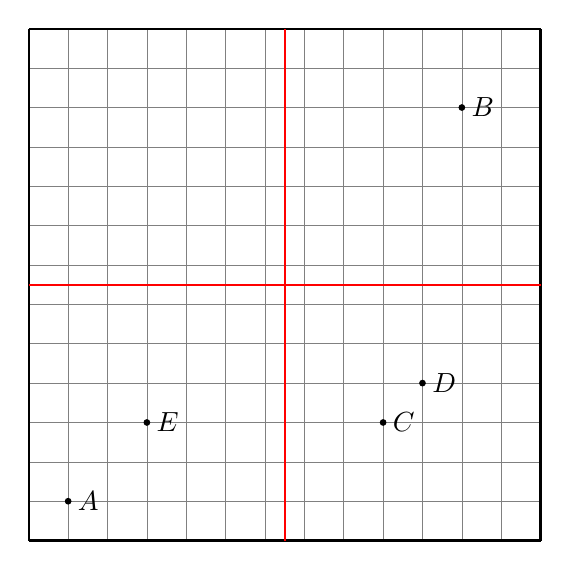
\begin{tikzpicture}
				\draw[step=0.5cm,gray,very thin] (-1,-1) grid (5.5,5.5);
				\draw[thick,-] (-1,-1) -- (5.5,-1);
				\draw[thick,-] (5.5,-1) -- (5.5,5.5);
				\draw[thick,-] (5.5,5.5) -- (-1,5.5);
				\draw[thick,-] (-1,5.5) -- (-1,-1);
				\filldraw[black] (-0.5,-0.5) circle (1pt) node[anchor=west]{$A$};
				\filldraw[black] (4.5,4.5) circle (1pt) node[anchor=west]{$B$};
				\filldraw[black] (3.5,0.5) circle (1pt) node[anchor=west]{$C$};
				\filldraw[black] (4,1) circle (1pt) node[anchor=west]{$D$};
				\filldraw[black] (0.5,0.5) circle (1pt) node[anchor=west]{$E$};
				\draw[thick,-, red] (-1,2.25) -- (5.5,2.25);
				\draw[thick,-, red] (2.25,-1) -- (2.25,5.5);
			\end{tikzpicture}
		\end{center}
	\end{frame}
	\begin{frame}{After the quad-split, we are able to add $F,G,H$, and $I$ to the Quad tree without overflow.}
		\begin{center}
			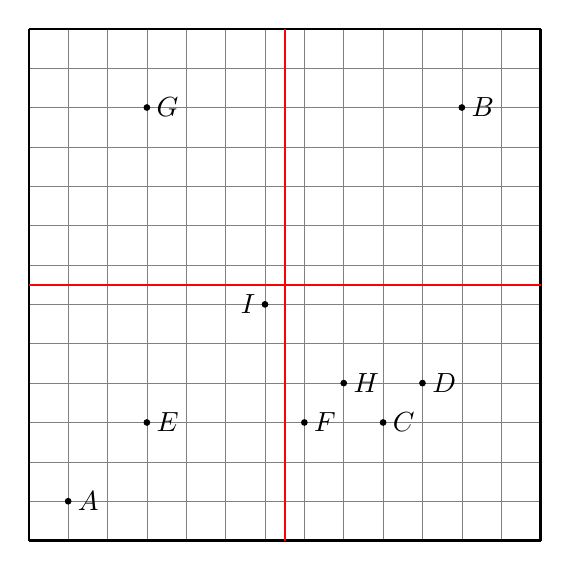
\begin{tikzpicture}
				\draw[step=0.5cm,gray,very thin] (-1,-1) grid (5.5,5.5);
				\draw[thick,-] (-1,-1) -- (5.5,-1);
				\draw[thick,-] (5.5,-1) -- (5.5,5.5);
				\draw[thick,-] (5.5,5.5) -- (-1,5.5);
				\draw[thick,-] (-1,5.5) -- (-1,-1);
				\filldraw[black] (-0.5,-0.5) circle (1pt) node[anchor=west]{$A$};
				\filldraw[black] (4.5,4.5) circle (1pt) node[anchor=west]{$B$};
				\filldraw[black] (3.5,0.5) circle (1pt) node[anchor=west]{$C$};
				\filldraw[black] (4,1) circle (1pt) node[anchor=west]{$D$};
				\filldraw[black] (0.5,0.5) circle (1pt) node[anchor=west]{$E$};
				\draw[thick,-, red] (-1,2.25) -- (5.5,2.25);
				\draw[thick,-, red] (2.25,-1) -- (2.25,5.5);
				\filldraw[black] (2.5,0.5) circle (1pt) node[anchor=west]{$F$};
				\filldraw[black] (0.5,4.5) circle (1pt) node[anchor=west]{$G$};
				\filldraw[black] (3,1) circle (1pt) node[anchor=west]{$H$};
				\filldraw[black] (2,2) circle (1pt) node[anchor=east]{$I$};
				
			\end{tikzpicture}
		\end{center}
	\end{frame}
	\begin{frame}{{\bf Overflow!} Adding Point $J$, means that we will have 5 points in the Southeast quadrant which is higher than 4. Therefore we have to do a quad-split on just the SE quadrant. }
		\begin{center}
			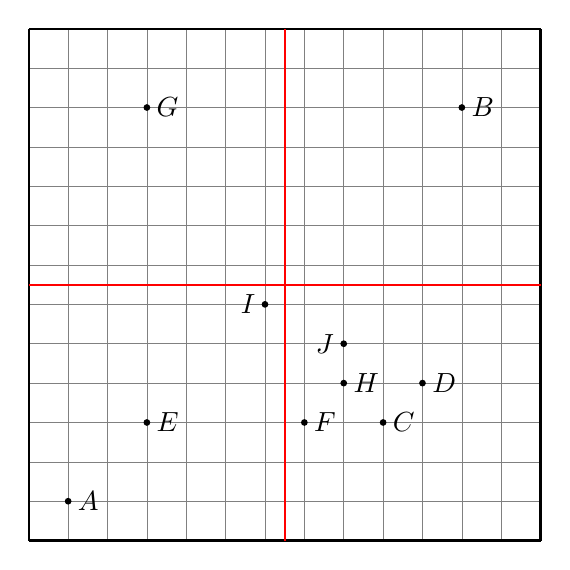
\begin{tikzpicture}
				\draw[step=0.5cm,gray,very thin] (-1,-1) grid (5.5,5.5);
				\draw[thick,-] (-1,-1) -- (5.5,-1);
				\draw[thick,-] (5.5,-1) -- (5.5,5.5);
				\draw[thick,-] (5.5,5.5) -- (-1,5.5);
				\draw[thick,-] (-1,5.5) -- (-1,-1);
				\filldraw[black] (-0.5,-0.5) circle (1pt) node[anchor=west]{$A$};
				\filldraw[black] (4.5,4.5) circle (1pt) node[anchor=west]{$B$};
				\filldraw[black] (3.5,0.5) circle (1pt) node[anchor=west]{$C$};
				\filldraw[black] (4,1) circle (1pt) node[anchor=west]{$D$};
				\filldraw[black] (0.5,0.5) circle (1pt) node[anchor=west]{$E$};
				\draw[thick,-, red] (-1,2.25) -- (5.5,2.25);
				\draw[thick,-, red] (2.25,-1) -- (2.25,5.5);
				\filldraw[black] (2.5,0.5) circle (1pt) node[anchor=west]{$F$};
				\filldraw[black] (0.5,4.5) circle (1pt) node[anchor=west]{$G$};
				\filldraw[black] (3,1) circle (1pt) node[anchor=west]{$H$};
				\filldraw[black] (2,2) circle (1pt) node[anchor=east]{$I$};
				\filldraw[black] (3,1.5) circle (1pt) node[anchor=east]{$J$};
			\end{tikzpicture}
		\end{center}
	\end{frame}
		\begin{frame}{Again, we bisect length and width to separate the SE quadrant. Lastly, we have no more points to add and all boxes have less than 4 points. {\bf DONE! :)}}
		\begin{center}
			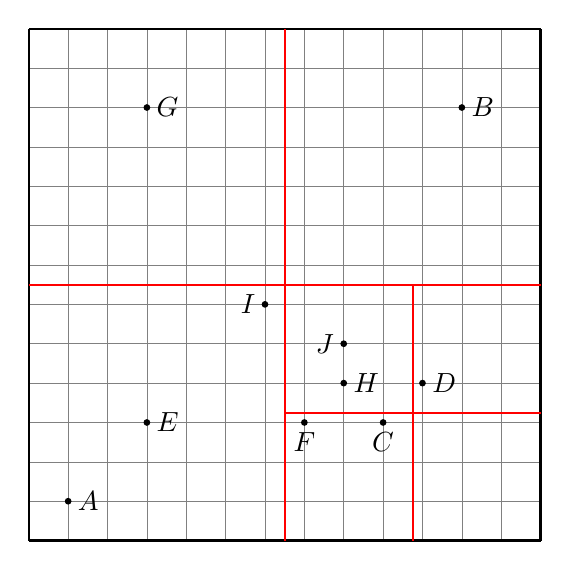
\begin{tikzpicture}
				\draw[step=0.5cm,gray,very thin] (-1,-1) grid (5.5,5.5);
				\draw[thick,-] (-1,-1) -- (5.5,-1);
				\draw[thick,-] (5.5,-1) -- (5.5,5.5);
				\draw[thick,-] (5.5,5.5) -- (-1,5.5);
				\draw[thick,-] (-1,5.5) -- (-1,-1);
				\filldraw[black] (-0.5,-0.5) circle (1pt) node[anchor=west]{$A$};
				\filldraw[black] (4.5,4.5) circle (1pt) node[anchor=west]{$B$};
				\filldraw[black] (3.5,0.5) circle (1pt) node[anchor=north]{$C$};
				\filldraw[black] (4,1) circle (1pt) node[anchor=west]{$D$};
				\filldraw[black] (0.5,0.5) circle (1pt) node[anchor=west]{$E$};
				\draw[thick,-, red] (-1,2.25) -- (5.5,2.25);
				\draw[thick,-, red] (2.25,-1) -- (2.25,5.5);
				\filldraw[black] (2.5,0.5) circle (1pt) node[anchor=north]{$F$};
				\filldraw[black] (0.5,4.5) circle (1pt) node[anchor=west]{$G$};
				\filldraw[black] (3,1) circle (1pt) node[anchor=west]{$H$};
				\filldraw[black] (2,2) circle (1pt) node[anchor=east]{$I$};
				\filldraw[black] (3,1.5) circle (1pt) node[anchor=east]{$J$};
				\draw[thick,-, red] (3.875,-1) -- (3.875,2.25);
				\draw[thick,-, red] (2.25, 0.625) -- (5.5,0.625);
			\end{tikzpicture}
		\end{center}
	\end{frame}
	
	\section{Assignment 4-2: kD-Trees}
		\begin{frame}{kd-Tree Set-up}
		Insert the following points (in this order) into an initially empy Quad-Tree:
		\begin{align*}
			A = (0,0), B = (10,10), C &= (8,2), D = (9,3), E = (2,2),\\
			F = (6,2), G = (2,10), H &= (7,3), I = (5,5), J = (7,4)
		\end{align*}
		The maximum page capacity of this kd-Tree is 4.
		\begin{itemize}
			\item Draw the current kd-tree after each split.
		\end{itemize}
	\end{frame}
		\begin{frame}{The initially empty kd-tree has one entry that covers the entire data space, by definition. We decided to make it $[-1,12]\times [-1,12]$.}
		\begin{center}
			
\begin{tikzpicture}
				\draw[step=0.5cm,gray,very thin] (-1,-1) grid (5.5,5.5);
				\draw[thick,-] (-1,-1) -- (5.5,-1);
				\draw[thick,-] (5.5,-1) -- (5.5,5.5);
				\draw[thick,-] (5.5,5.5) -- (-1,5.5);
				\draw[thick,-] (-1,5.5) -- (-1,-1);
			\end{tikzpicture}
		\end{center}
		
	\end{frame}
	\begin{frame}{Since the page capacity is 4, we are able to add $A,B,C,$ and $D$ with no hiccups.}
		\begin{center}
			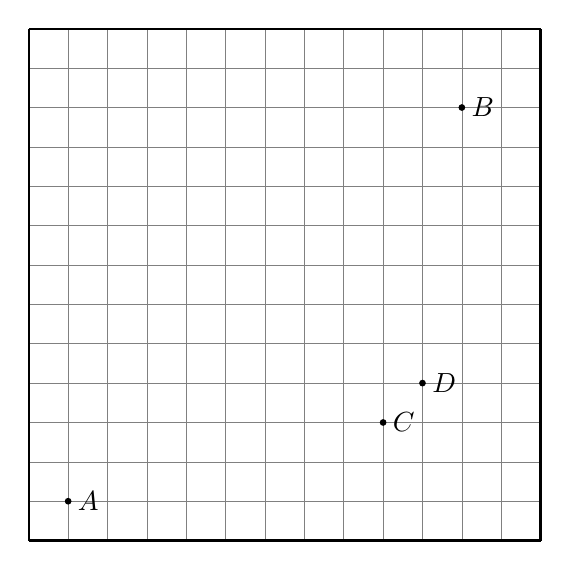
\begin{tikzpicture}
				\draw[step=0.5cm,gray,very thin] (-1,-1) grid (5.5,5.5);
				\draw[thick,-] (-1,-1) -- (5.5,-1);
				\draw[thick,-] (5.5,-1) -- (5.5,5.5);
				\draw[thick,-] (5.5,5.5) -- (-1,5.5);
				\draw[thick,-] (-1,5.5) -- (-1,-1);
				\filldraw[black] (-0.5,-0.5) circle (1pt) node[anchor=west]{$A$};
				\filldraw[black] (4.5,4.5) circle (1pt) node[anchor=west]{$B$};
				\filldraw[black] (3.5,0.5) circle (1pt) node[anchor=west]{$C$};
				\filldraw[black] (4,1) circle (1pt) node[anchor=west]{$D$};
			\end{tikzpicture}
		\end{center}
	\end{frame}
		\begin{frame}{{\bf Overflow!} Adding Point $E$, means that we will have 5 points in the data space, which is higher than 4. Since depth(Point $E$) \% 2 = 0, we will perform a horizontal split.} 
		\begin{center}
			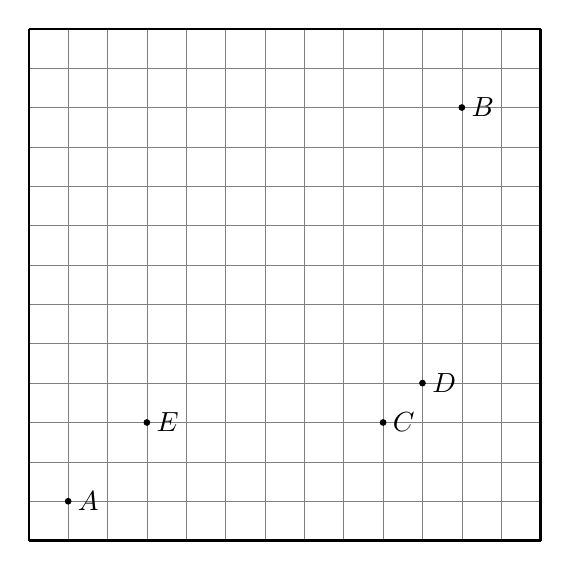
\begin{tikzpicture}
				\draw[step=0.5cm,gray,very thin] (-1,-1) grid (5.5,5.5);
				\draw[thick,-] (-1,-1) -- (5.5,-1);
				\draw[thick,-] (5.5,-1) -- (5.5,5.5);
				\draw[thick,-] (5.5,5.5) -- (-1,5.5);
				\draw[thick,-] (-1,5.5) -- (-1,-1);
				\filldraw[black] (-0.5,-0.5) circle (1pt) node[anchor=west]{$A$};
				\filldraw[black] (4.5,4.5) circle (1pt) node[anchor=west]{$B$};
				\filldraw[black] (3.5,0.5) circle (1pt) node[anchor=west]{$C$};
				\filldraw[black] (4,1) circle (1pt) node[anchor=west]{$D$};
				\filldraw[black] (0.5,0.5) circle (1pt) node[anchor=west]{$E$};
			\end{tikzpicture}
		\end{center}
	\end{frame}
	\begin{frame}{We need to make sure that the vertical line separates the points around the median, so there are 2 points on one side, 3 on the other.} 
		\begin{center}
			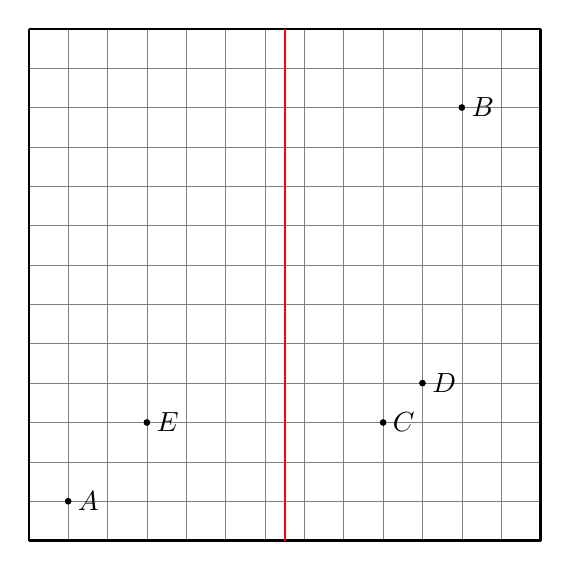
\begin{tikzpicture}
				\draw[step=0.5cm,gray,very thin] (-1,-1) grid (5.5,5.5);
				\draw[thick,-] (-1,-1) -- (5.5,-1);
				\draw[thick,-] (5.5,-1) -- (5.5,5.5);
				\draw[thick,-] (5.5,5.5) -- (-1,5.5);
				\draw[thick,-] (-1,5.5) -- (-1,-1);
				\filldraw[black] (-0.5,-0.5) circle (1pt) node[anchor=west]{$A$};
				\filldraw[black] (4.5,4.5) circle (1pt) node[anchor=west]{$B$};
				\filldraw[black] (3.5,0.5) circle (1pt) node[anchor=west]{$C$};
				\filldraw[black] (4,1) circle (1pt) node[anchor=west]{$D$};
				\filldraw[black] (0.5,0.5) circle (1pt) node[anchor=west]{$E$};
				\draw[thick,-, red] (2.25, -1) -- (2.25,5.5);
			\end{tikzpicture}
		\end{center}
	\end{frame}
	\begin{frame}{We can add Points $F$ and $G$ to the kd-tree, and both nodes still have $\leq 4$ points.} 
		\begin{center}
			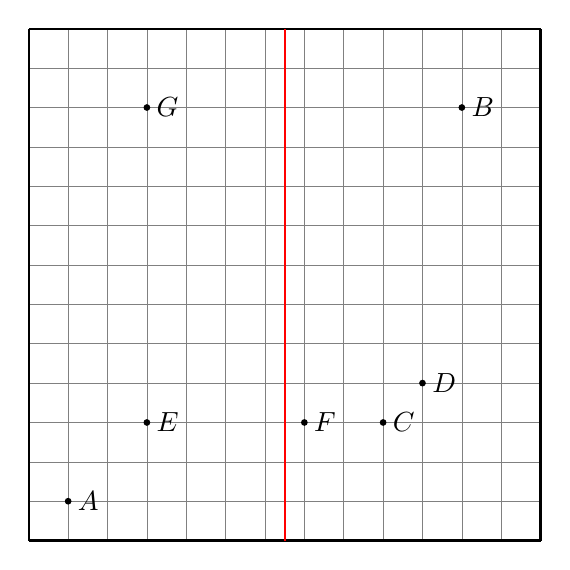
\begin{tikzpicture}
				\draw[step=0.5cm,gray,very thin] (-1,-1) grid (5.5,5.5);
				\draw[thick,-] (-1,-1) -- (5.5,-1);
				\draw[thick,-] (5.5,-1) -- (5.5,5.5);
				\draw[thick,-] (5.5,5.5) -- (-1,5.5);
				\draw[thick,-] (-1,5.5) -- (-1,-1);
				\filldraw[black] (-0.5,-0.5) circle (1pt) node[anchor=west]{$A$};
				\filldraw[black] (4.5,4.5) circle (1pt) node[anchor=west]{$B$};
				\filldraw[black] (3.5,0.5) circle (1pt) node[anchor=west]{$C$};
				\filldraw[black] (4,1) circle (1pt) node[anchor=west]{$D$};
				\filldraw[black] (0.5,0.5) circle (1pt) node[anchor=west]{$E$};
				\draw[thick,-, red] (2.25, -1) -- (2.25,5.5);
				\filldraw[black] (2.5,0.5) circle (1pt) node[anchor=west]{$F$};
				\filldraw[black] (0.5,4.5) circle (1pt) node[anchor=west]{$G$};
			\end{tikzpicture}
		\end{center}
	\end{frame}
		\begin{frame}{{\bf Overflow!} Adding Point $H$, means that we will have 5 points in theright node, which is higher than 4. Since depth(Point $H$) \% 2 = 1, we will perform a vertical split.} 
		\begin{center}
			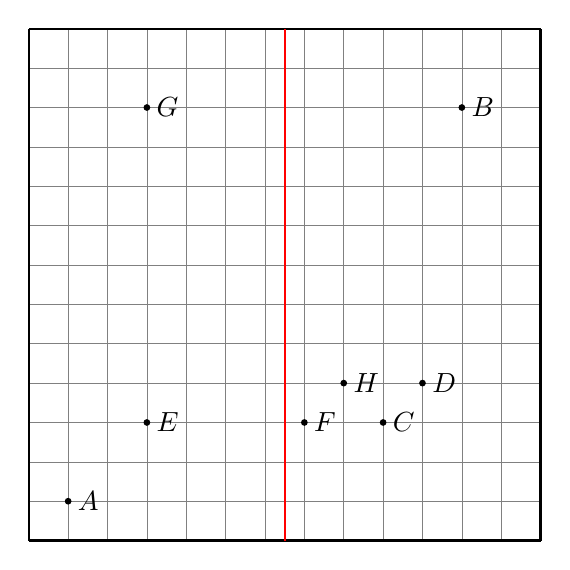
\begin{tikzpicture}
				\draw[step=0.5cm,gray,very thin] (-1,-1) grid (5.5,5.5);
				\draw[thick,-] (-1,-1) -- (5.5,-1);
				\draw[thick,-] (5.5,-1) -- (5.5,5.5);
				\draw[thick,-] (5.5,5.5) -- (-1,5.5);
				\draw[thick,-] (-1,5.5) -- (-1,-1);
				\filldraw[black] (-0.5,-0.5) circle (1pt) node[anchor=west]{$A$};
				\filldraw[black] (4.5,4.5) circle (1pt) node[anchor=west]{$B$};
				\filldraw[black] (3.5,0.5) circle (1pt) node[anchor=west]{$C$};
				\filldraw[black] (4,1) circle (1pt) node[anchor=west]{$D$};
				\filldraw[black] (0.5,0.5) circle (1pt) node[anchor=west]{$E$};
				\draw[thick,-, red] (2.25, -1) -- (2.25,5.5);
				\filldraw[black] (2.5,0.5) circle (1pt) node[anchor=west]{$F$};
				\filldraw[black] (0.5,4.5) circle (1pt) node[anchor=west]{$G$};
				\filldraw[black] (3,1) circle (1pt) node[anchor=west]{$H$};
			\end{tikzpicture}
		\end{center}
	\end{frame}
	\begin{frame}{We need to make sure that the horizontal line separates the points around the median, so there are 2 points on one side, 3 on the other.} 
		\begin{center}
			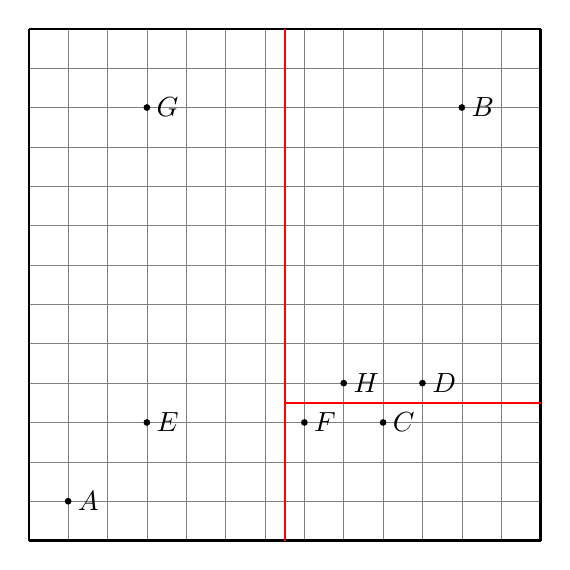
\begin{tikzpicture}
				\draw[step=0.5cm,gray,very thin] (-1,-1) grid (5.5,5.5);
				\draw[thick,-] (-1,-1) -- (5.5,-1);
				\draw[thick,-] (5.5,-1) -- (5.5,5.5);
				\draw[thick,-] (5.5,5.5) -- (-1,5.5);
				\draw[thick,-] (-1,5.5) -- (-1,-1);
				\filldraw[black] (-0.5,-0.5) circle (1pt) node[anchor=west]{$A$};
				\filldraw[black] (4.5,4.5) circle (1pt) node[anchor=west]{$B$};
				\filldraw[black] (3.5,0.5) circle (1pt) node[anchor=west]{$C$};
				\filldraw[black] (4,1) circle (1pt) node[anchor=west]{$D$};
				\filldraw[black] (0.5,0.5) circle (1pt) node[anchor=west]{$E$};
				\draw[thick,-, red] (2.25, -1) -- (2.25,5.5);
				\filldraw[black] (2.5,0.5) circle (1pt) node[anchor=west]{$F$};
				\filldraw[black] (0.5,4.5) circle (1pt) node[anchor=west]{$G$};
				\filldraw[black] (3,1) circle (1pt) node[anchor=west]{$H$};
				\draw[thick,-, red] (2.25, 0.75) -- (5.5,0.75);
			\end{tikzpicture}
		\end{center}
	\end{frame}
		\begin{frame}{We add Points $I$ and $J$ to the kd-Tree. Lastly, we have no more points to add and all nodes have $\leq4$ points. {\bf DONE! :)}} 
		\begin{center}
			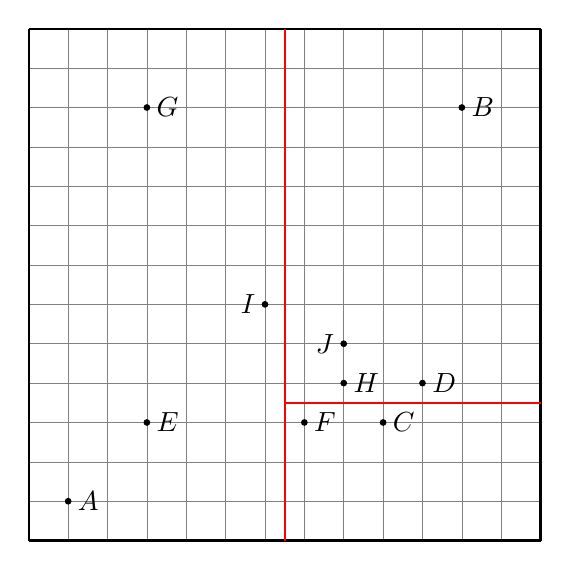
\begin{tikzpicture}
				\draw[step=0.5cm,gray,very thin] (-1,-1) grid (5.5,5.5);
				\draw[thick,-] (-1,-1) -- (5.5,-1);
				\draw[thick,-] (5.5,-1) -- (5.5,5.5);
				\draw[thick,-] (5.5,5.5) -- (-1,5.5);
				\draw[thick,-] (-1,5.5) -- (-1,-1);
				\filldraw[black] (-0.5,-0.5) circle (1pt) node[anchor=west]{$A$};
				\filldraw[black] (4.5,4.5) circle (1pt) node[anchor=west]{$B$};
				\filldraw[black] (3.5,0.5) circle (1pt) node[anchor=west]{$C$};
				\filldraw[black] (4,1) circle (1pt) node[anchor=west]{$D$};
				\filldraw[black] (0.5,0.5) circle (1pt) node[anchor=west]{$E$};
				\draw[thick,-, red] (2.25, -1) -- (2.25,5.5);
				\filldraw[black] (2.5,0.5) circle (1pt) node[anchor=west]{$F$};
				\filldraw[black] (0.5,4.5) circle (1pt) node[anchor=west]{$G$};
				\filldraw[black] (3,1) circle (1pt) node[anchor=west]{$H$};
				\draw[thick,-, red] (2.25, 0.75) -- (5.5,0.75);
				\filldraw[black] (2,2) circle (1pt) node[anchor=east]{$I$};
				\filldraw[black] (3,1.5) circle (1pt) node[anchor=east]{$J$};
			\end{tikzpicture}
		\end{center}
	\end{frame}
	
	\section{Assignment 4-4: R Trees}
\begin{frame}{This is the R-tree into which we are inserting points.} 
\begin{center}
	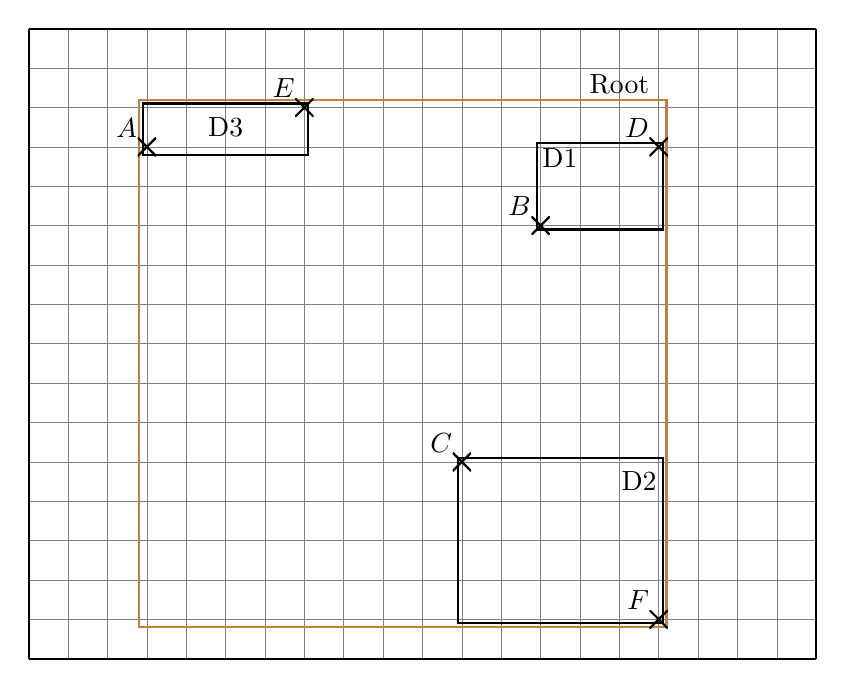
\begin{tikzpicture}
		\draw[step=0.5cm,gray,very thin] (0,0) grid (10,8);
		\draw[thick,-] (0,0) -- (10,0);
		\draw[thick,-] (10,0) -- (10,8);
		\draw[thick,-] (10,8) -- (0,8);
		\draw[thick,-] (0,8) -- (0,0);
		\draw[brown, thick] (1.4,0.4) rectangle (8.1,7.1);
		\draw (7.5,7.3) node {Root};
		\node[cross,thick,minimum size=1pt] at (1.5,6.5) {};
		\draw (1.5,6.5) node[anchor = south east] {$A$};
		\node[cross,thick,minimum size=1pt] at (3.5,7) {};
		\draw (3.5,7) node[anchor = south east] {$E$};
		\draw[black, thick] (1.45,6.4) rectangle (3.55,7.05);
		\draw (2.5,6.75) node {D3};
		\node[cross,thick,minimum size=1pt] at (8,0.5) {};
		\draw (8.0,0.5) node[anchor = south east] {$F$};
		\node[cross,thick,minimum size=1pt] at (5.5,2.5) {};
		\draw (5.5,2.5) node[anchor = south east] {$C$};
		\draw[black, thick] (5.45,0.45) rectangle (8.05,2.55);
		\draw (7.75,2.25) node {D2};
		\node[cross,thick,minimum size=1pt] at (8,6.5) {};
		\draw (8,6.5) node[anchor = south east] {$D$};
		\node[cross,thick,minimum size=1pt] at (6.5,5.5) {};
		\draw (6.5,5.5) node[anchor = south east] {$B$};
		\draw[black, thick] (6.45,5.45) rectangle (8.05,6.55);
		\draw (6.4,6.6) node[anchor = north west] {D1};
	\end{tikzpicture}
\end{center}
\end{frame}
\begin{frame}{We are able to add Points $G$ and $H$ into their nodes without overflow.} 
	\begin{center}
		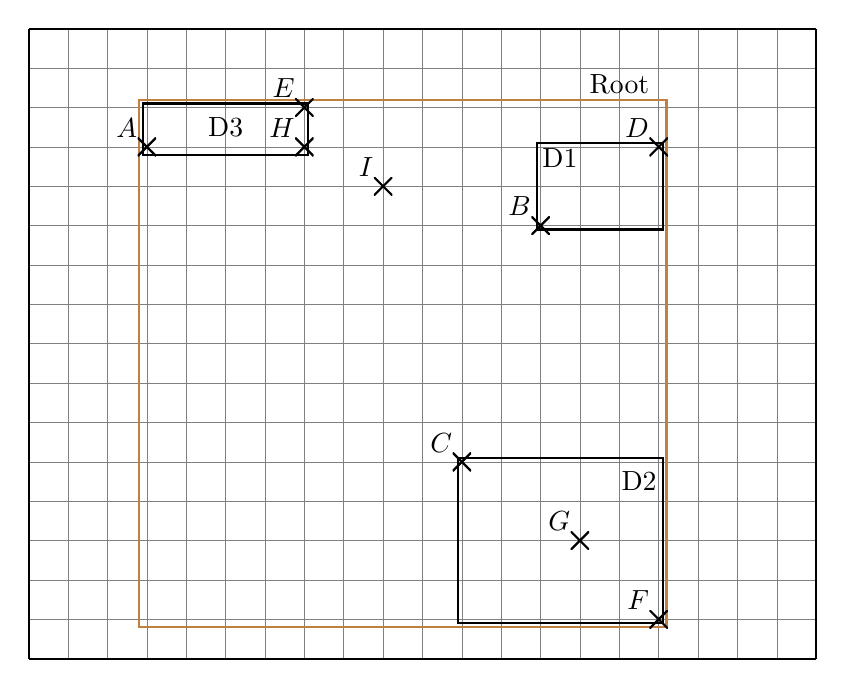
\begin{tikzpicture}
			\draw[step=0.5cm,gray,very thin] (0,0) grid (10,8);
			\draw[thick,-] (0,0) -- (10,0);
			\draw[thick,-] (10,0) -- (10,8);
			\draw[thick,-] (10,8) -- (0,8);
			\draw[thick,-] (0,8) -- (0,0);
			\draw[brown, thick] (1.4,0.4) rectangle (8.1,7.1);
			\draw (7.5,7.3) node {Root};
			\node[cross,thick,minimum size=1pt] at (1.5,6.5) {};
			\draw (1.5,6.5) node[anchor = south east] {$A$};
			\node[cross,thick,minimum size=1pt] at (3.5,7) {};
			\draw (3.5,7) node[anchor = south east] {$E$};
			\draw[black, thick] (1.45,6.4) rectangle (3.55,7.05);
			\draw (2.5,6.75) node {D3};
			\node[cross,thick,minimum size=1pt] at (8,0.5) {};
			\draw (8.0,0.5) node[anchor = south east] {$F$};
			\node[cross,thick,minimum size=1pt] at (5.5,2.5) {};
			\draw (5.5,2.5) node[anchor = south east] {$C$};
			\draw[black, thick] (5.45,0.45) rectangle (8.05,2.55);
			\draw (7.75,2.25) node {D2};
			\node[cross,thick,minimum size=1pt] at (8,6.5) {};
			\draw (8,6.5) node[anchor = south east] {$D$};
			\node[cross,thick,minimum size=1pt] at (6.5,5.5) {};
			\draw (6.5,5.5) node[anchor = south east] {$B$};
			\draw[black, thick] (6.45,5.45) rectangle (8.05,6.55);
			\draw (6.4,6.6) node[anchor = north west] {D1};
			% New points G
			\node[cross,thick,minimum size=1pt] at (7,1.5) {};
			\draw (7,1.5) node[anchor = south east] {$G$};
			% New points H
			\node[cross,thick,minimum size=1pt] at (3.5,6.5) {};
			\draw (3.5,6.5) node[anchor = south east] {$H$};
			% New points I
			\node[cross,thick,minimum size=1pt] at (4.5,6) {};
			\draw (4.5,6) node[anchor = south east] {$I$};
		\end{tikzpicture}
	\end{center}
\end{frame}
	

\end{document}
